\newpage
\section{Regresión Lineal Tarea}
\subsection{Enunciado}
\textbf{A:} Completar la segunda parte del modelo lineal presentado en clases.
\begin{figure}[h!]
    \centering
    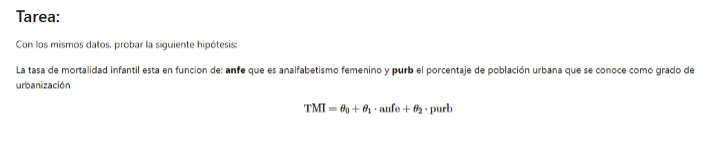
\includegraphics[width=1\textwidth]{images/statement.png}
    \caption{Enunciado de regresión lineal}
    \label{fig:regresion_lineal_statement}
\end{figure}

\begin{verbatim}
municipios = pd.read_csv('mun_cbba/Mun_Cbba2.csv', sep=';', decimal=',')
modelo = smf.ols(formula="tmi ~ anfe + purb", data=municipios).fit()

residuos = modelo.resid
stats.probplot(residuos, dist="norm", plot=plt)
plt.title("Gráfico Q-Q de los Residuos")
plt.show()

stat, p_value = shapiro(residuos)
print('Estadístico de Shapiro-Wilk:', stat)
print('p-value:', p_value)

print(modelo.summary())
\end{verbatim}

Del resultado el modelo considerando los coeficientes se obtiene que el modelo es:
$$
TMI = 34.1012 + 1.3292 \cdot anfe + 0.0505 \cdot purb
$$



Se realiza una evaluación teórica.

Se planteó que las condiciones de vida y el grado de urbanización implicaban un impacto sobre la mortalidad infantil:

a) Mayor tasa de analfabetismo femenino (anfe) 
implica una mayor tasa de mortalidad infantil.
El signo del coeficiente debe ser positivo. En el modelo estimado, 
el coeficiente de anfe anfe es  1.3292 1.3292, lo cual es consistente con la teoría. 
Este coeficiente es estadísticamente significativo ( p < 0.001 p<0.001), 
lo que indica que existe evidencia empírica para concluir que el analfabetismo 
femenino tiene un impacto positivo y significativo sobre la mortalidad infantil.

b) Mayor porcentaje de población urbana (purb) 
implica una mayor tasa de mortalidad infantil. 
El signo del coeficiente también debe ser positivo. 
En el modelo estimado, el coeficiente de purb purb es  
0.0505 0.0505, pero este valor no es estadísticamente significativo 
( p = 0.588 > 0.05 p=0.588>0.05). 
Esto sugiere que no hay evidencia empírica suficiente para concluir 
que el grado de urbanización afecta significativamente la mortalidad infantil.

El modelo estimado constituye una evidencia empírica parcial de la teoría planteada en el primer paso: mientras que el analfabetismo femenino demuestra ser un factor significativo, el grado de urbanización no tiene un impacto concluyente en este caso.



Evaluacion de la bondad de ajuste

En este ejemplo, el indicador es R2 = 0.726 
R2=0.726, lo que significa que el 72.6\% de la variabilidad de la 
mortalidad infantil está explicada por la asociación lineal 
con el analfabetismo femenino ( anfe anfe) y el grado de urbanización ( purb).
El restante 27.4\% 
se debe a otros factores no considerados en este modelo.

\section{Regresión Lineal Base de Datos}
\subsection{Enunciado}
Generar una regresión lineal múltiple con 3 variables: dos  independiente y 1 dependientes (variable target, objetivo). Puede usar las bases de datos reales que uso en las prácticas anteriores  (10 Puntos)

\subsection{Hipótesis}
Hipótesis: La tasa de rotación de empleados está relacionada con: \\


\textbf{Hipótesis:} La tasa de rotación de empleados está en función de los años totales de experiencia laboral (TotalWorkingYears) y el equilibrio entre la vida laboral y personal (WorkLifeBalance).

\textbf{Modelo Estimado:} 
\[
\textbf{Attrition} = -0.1566 + -0.0911 \cdot \textbf{TotalWorkingYears} + -0.2026 \cdot \textbf{WorkLifeBalance}
\]

\textbf{Interpretación de los Coeficientes:}
\begin{itemize}
    \item \textbf{TotalWorkingYears}: Por cada año adicional de experiencia laboral, el logaritmo de las probabilidades de rotación cambia en -0.0911. 
    \item \textbf{WorkLifeBalance}: Por cada nivel adicional de equilibrio trabajo-vida, el logaritmo de las probabilidades de rotación cambia en -0.2026.
\end{itemize}


\textbf{Evaluación del Modelo:}
\begin{itemize}
    \item \textbf{Precisión del modelo:} 0.8617
    \item \textbf{Recall (Yes):} 0.0000 (Sensibilidad para detectar empleados que dejan la empresa).
    \item \textbf{Precision (Yes):} 0.0000 (Precisión para predecir empleados que dejan la empresa).
\end{itemize}